%% Credits of this ams template are with respective people. @Devansh1106 neither own this template nor the credits. 
\documentclass[reqno,10pt]{amsart}
\usepackage[a4paper, margin=1.25in]{geometry} % Change 1in to desired size
\usepackage[numbers]{natbib}
\setlength{\bibsep}{8pt}
\usepackage{dsfont}
\usepackage{graphicx}
\usepackage{tikz-cd}
\usepackage{subcaption}
% \captionsetup[subfigure]{labelformat=parens,labelfont=normalfont}
% \renewcommand{\thesubfigure}{\alph{subfigure}}
\usepackage{hyperref}
\usepackage{lineno}
\usepackage{amssymb}
\usepackage{amsmath}
\usepackage{amsthm}
\usepackage{mathtools}
\usepackage{mathrsfs}
\usepackage{esint}
\usepackage{fancyhdr}

\DeclareMathAlphabet{\EuScript}{U}{eus}{m}{n}

\setlength{\parskip}{0.5\baselineskip}%
\setlength{\parindent}{20pt}
\theoremstyle{plain}

\pagestyle{fancy}
\fancyhf{} % Clear default headers/footers
\setlength{\headheight}{10.0pt}
% Even pages: Paper title
\fancyhead[LE]{\footnotesize\textit{Universality of POSEIDON in settings of ANOs}}

% Odd pages: Author name
\fancyhead[RO]{\footnotesize\textit{Devansh Tripathi}}

\newtheorem*{thm*}{Theorem}
%% this allows for theorems which are not automatically numbered
\newcommand{\sinc}{\text{sinc}}
\renewcommand{\qedsymbol}{$\blacksquare$}
\newtheorem{thm}{Theorem}
\newtheorem{cor}{Corollary}
\newtheorem{lem}{Lemma}
\newtheorem*{lem*}{Lemma}
\newtheorem{prop}{Proposition}
\theoremstyle{definition}
\newtheorem{defn}{Definition}
\newtheorem{eg}{Example}
\newtheorem{rem}{Remark}
\newcommand{\bb}[1]{\mathbb{#1}}
\newcommand{\cal}[1]{\mathcal{#1}}
\newcommand{\eus}[1]{\EuScript{#1}}

\hypersetup{
    colorlinks=false,
    linkcolor=blue,    % Internal links (sections, equations)
    citecolor=red,     % Citation links
    urlcolor=magenta   % URLs (DOIs, websites)
}
%% The above lines are for formatting.  In general, you will not want to change these.

\title{Report on the paper ``Geometry Aware Operator Transformer As An Efficient And Accurate Neural Surrogate For PDEs On Arbitrary Domains''}
\author{Devansh Tripathi$^1$ \\ ETH Z\lowercase{\"urich}}
\thanks{$^1$Seminar für Angewandte Mathematik, HG E 62.2, Rämistrasse 101, 8092 Zürich, Switzerland \\ \href{mailto:devansh.tripathi@sam.math.ethz.ch}{\texttt{devansh.tripathi@sam.math.ethz.ch}}}

\begin{document}
\numberwithin{equation}{section}

\begin{abstract}
    In this paper \cite{SW2025}, the authors address the pressing issue in the realm of operator learning that many of the accurate models are not computaionally efficient and vice versa. They propose a geometry aware operator transformer (GAOT)(pronounced goat) for learning PDEs on arbitrary domains which is computaionally efficient as well as accurate. GAOT combines novel multiscale attentional graph neural operator encoders and decoders, together with geometry embeddings and (vision) transformer processors. With multiple innovations in the implementations of GAOT to ensure computational efficieny and scalability, GAOT achieves state of the art performance on a large 3D industrial CFD dataset. 
\end{abstract}
\maketitle
\section{\bf Contributions of the paper}
Authors proposes a {\it Geometry Aware Operator Transformer} (GAOT, pronounced goat) as a neural surrogate for PDEs on arbitrary domains. While being based on the well-established {\it encode-process-decode} paradigm, GAOT includes several novel features that are designed to ensure both computational efficieny and accuracy, such as

\begin{itemize}\setlength{\itemsep}{0.7em}
    \item Our proposed {\it multiscale attentional graph neural operator} (MAGNO) as the encoder between inputs on an arbitrary point cloud and a {\it coarser} latent grid, designed to enhance accuracy through its multiscale information processing and attention modules.
    \item Novel {\it Geometry embeddings} in the encoder (and decoder) that provides the model with access to information about the (local) domain geometry, greatly increasing accuracy. 
    \item A {\it transformer processor} that utilizes patching (as in ViT \cite{AD2021}) for computational efficieny.
    \item A MAGNO decoder, able to generate {\it neural fields}, with the ability to approximate the underlying solution at {\it any query point} in the domain.
    \item A set of implementation strategies to ensure that the computational realization of GAOT is efficient and highly scalable.
\end{itemize}
The demonstration of these capabilities is by,

\begin{itemize}\setlength{\itemsep}{0.7em}
    \item Extensively testing GAOT on 24 challenging benchmarks for both timw-independent and time-dependent PDEs of various types, ranging from regular grids to random point clouds to highly instructured adapted grids, and comparing it with widely-used baselines to show that GAOT is both highly accurate as well as computationally efficient and scalable.
    \item The efficiency and scalability of GAOT is further showcased by it achieving state of the art (SOTA) performance on the large scale 3D industrial benchmark of {\it DrivAerNet++} dataset for automobile aerodynamics \cite{ME2025}.
    \item Through extensive ablations, we also highlight how the novel elements in the design of GAOT such as multiscale attentional encoders and geometry embeddings crucially contribute to the overall performance of our model.
\end{itemize}

\section{\bf Methods}
\paragraph{\bf Problem Formulation} We start with a generic {\it time-independent} PDE,
\begin{equation}\label{eq:pde}
    \cal D(c,u) = f, \qquad \forall x  \in D\subset \bb R^d, \qquad \cal B(u) = u_b, \qquad x\in \partial D,
\end{equation}
with $u: D \to \bb R^m$, the PDE solution, $c$ is the coefficient (PDE parameters), $f$ is the forcing term, $u_b$ are the boundary values and $\cal D$ and $\cal B$ are the underlying differential and boundary operators, respectively. Denoting as $\chi_D$, a function (e.g. indicator or signed distance) parameterizing the domain $D$, we combine all the inputs to the PDE \ref{eq:pde} together into $a = (c,f,u_b,\chi_D)$, then the {\it solution operator} $\cal{S}$ maps inputs into PDE solution with $u = \cal S_a$. The corresponding {\it operator learning task} is to learn the solution operator $\cal S$ from data. To this end, let $\mu$ be an underlying {\it data distribution}. We sample i.i.d inputs $a^{(i)} \sim\mu$, for $1 \leq i \leq M$ and assume that we have access to {\it data pairs} $(s^{(i)}, u^{(i)})$ with $u^{(i)} = \cal Sa^{(i)}$, thus the operator learning task is to approximate the distribution $\cal S_{\#\mu}$ from these data pairs. 

\noindent Similarly denoting a generic {\it time-dependent} PDE as,
\begin{equation}\label{eq:tpde}
    u_t + \cal D(c,u) = 0, \quad \forall x \in D \subset \bb R^d, t \in [0,T] \quad u(0) = u_0, \quad x\in D
\end{equation}
with, $u : D \times [0,T] \mapsto \bb R^m$, $c$ the PDE coefficient and $u_0$ the initial datum and the underlying (spatial) differential operator $\cal D$. Clubbing the {\it inputs} to the PDE \ref{eq:tpde} into $a = (c,u_0,\chi_D)$, the corresponding {\it solution operator} $\cal S_t$, with $u(t) = \cal S_t(a)$ for all $t \in [0,T]$, maps the input into trajectory of the solution. The {\it operator learning task} consists of approximating $(\cal S_t)_{\#\mu}$ from the data pairs $(a^{(i)}, u^{(i)}(t))$ for all $t \in [0,T^{(i)}]$ and $1 \leq i \leq M$ with samples $a_i$ drawn from the data distribution $\mu$. However, in practice, we only have access to data, sampled on a discrete set of spatial points per sample as well as only on discrete time snapshots $t^{(i)}_n \in [0,T^{(i)}]$ and have to learn the solution from them.

\begin{figure}[!ht]
    \centering
    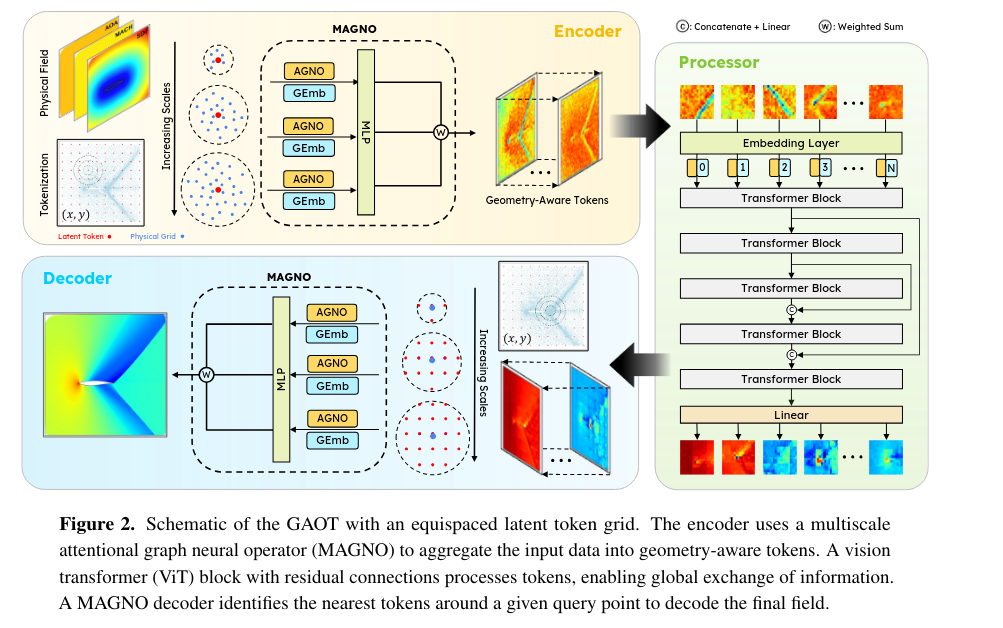
\includegraphics[width=\textwidth]{gaot_arch.png}
    \caption{Taken from \cite{SW2025}}
    \label{fig:gaot_arch}
\end{figure}

\paragraph{\bf GAOT Model Architecture} 
For simplicity, we start with the time-independent case, where given inputs $a(x_j)$ on the input cloud $D_\Delta = \{x_j\} \subset D,$ for $1 \leq j \leq J$, GAOT provides an approximation to solution $u$ of the PDE \ref{eq:pde} at any query point $x\in D$. In the first step, an {\it encoder} transforms the input on the underlying point cloud $D_\Delta$ to a {\it latent point cloud} $\cal D \subset \bb R^d$. The resulting {\it spatial tokens} are then processed by a processor module to learn useful representations and its output is remapped to the original domain $D$ via the {\it decoder}, which allows evaluation at any query point $x \in D$.

\paragraph{\bf Choice of Latent Domain} 
As shown in the figure in appendix \ref{appendix:lgrid}, the latent domain $\cal D$ (to which the encoder maps) can be chosen in three different ways, i) a regular (structured) grid stencil, consisting of equispaced points on a Cartesian domain ii) randomly downsampling the underlying point cloud $D_\Delta$ or iii) a projected low-dimensional representation, where a high-dimensional domain is projected to a lower dimension (for instance using tri-plane embeddings in 3D \cite{QC2025}) and a regular grid is used in the lower-dimension domain. GAOT is a general framework where any of these point cloud choices can be employed for $\cal D$.

\paragraph{\bf Encoder} Given input values $a(x_j)$ on the underlying point cloud $D_\Delta$, the encoder aims to transforms it into latent features $w_e(y)$ at any point $y \in \cal D$ on the latent point cloud. Using a graph-neural operator (GNO) encoder as in GINO \cite{ZL2023} would lead to,
\begin{equation}\label{eq:gno_single}
    \tilde{w}_e(y) = \sum_{k=1}^{n_y} \alpha_k K(y,x_k,a(x_k)) \varphi(a(x_k)),
\end{equation}
with MLPs $K$ and $\varphi$ and the sum above taken over all the $n_y$ points $x_k \in D_\Delta$ such that $|y-x_k| \leq r$ for some hyperparameter $r > 0$, where $\alpha_k$ are some given quadrature weights. In other words, GNO accumulates information from all the points in the original point cloud that lie inside a ball of radius $r$, centered at the given point $y$ in the latent point cloud, and processes them through a kernel integral.

\noindent Authors propose a mechanism to integrate {\it multiscale} information into the encoder. To this end, we choose $r_m = s_m r_0$, for some base radius $r_0$ and scale factors $s_m$, for $m = 1, \dots, \bar{m}$ to modify GNO \ref{eq:gno_single}, by,
\begin{equation}\label{eq:agno}
    \tilde{w}_e^m (y) = \sum_{k=1}^{n_y^m} \alpha_k^m K^m (y,x_k,a(x_k)) \varphi(a(x_k)),
\end{equation}
for any fixed scale $m$ and with MLPs $K^m. \varphi$. The above sum is taken over all the $n^m_y$ points $x_k \in D_\Delta$ such that $|y-x_k| \leq r_m$. To choose the quadrature weights $\alpha_k^m$, we propose an {\it attention based} choice,
\begin{equation}
    \alpha_k^m = \frac{\exp(e^m_k)}{\sum_{k'=1}^{n_y^m} \exp(e^m_{k'})}, \qquad e^m_k = \frac{\langle {\bf W}_q^m y,{\bf W}_\kappa^m x_k \rangle}{\sqrt{\overline{d}}},
\end{equation}
with ${\bf W}_q^m,{\bf W}_\kappa^m \in \bb R^{\overline{d} \times m}$ are query and key matrices respectively, completing the description of the {\it attentional graph neural operator} (AGNO) at each scale $m$.

\paragraph{\bf Geometry Embeddings}
The only geometric information in the afore-described encoder is provided by the coordinates of the underlying points. The authors argue that this alone does not convey the rich geometric information about the domain that can affect the solution of the underlying PDE \ref{eq:tpde}. In the literature, the geometry information is usually provided either by appending them as node and edge features on the underlying graphs or by encoding a signed distance function. The authors propose to use a novel {\it geometry embeddings} to encode this information. To this end as described in appendix \ref{appendix:gembedd}, we can rely on {\it local statistical embeddings} for each point $y \in \cal D$ as all the neighbouring points $x_k$ in $D_\Delta$ with $|y-x_k| \leq r_m$ have already been computed in the AGNO encoder. From these points, we can readily compute statistical descriptors such as i) number of neighbors $x_k \in D_\Delta$, in the ball $B_{r_m}(y)$, ii) the {\it average distance} $D_{avg} = \frac{1}{n_y^m} \sum_{k=1}^{n_y^m} |y-x_k|,$ iii) the variance of this distance $D_{var}$, with respect to the average $D_{avg}$, iv) the {\it centroid offset vector} $\Delta_y = \frac{1}{n_y^m} \sum_{k=1}^{n_x^y}(x_k-y)$ and v) a few principal component (PCA) features of the covariance matrix of $y-x_k$ to calculate the {\it local shape anisotropy}. These statistical descriptors, for each scale $m$ and each point $y \in \cal D$ are then concatenated into a single vector $z_y$, normalised across components to yield zero mean and unit variance and fed into an MLP to provide the embedding $g^m(y)$. Alternatively, geometry embedding using emphPointNet models \cite{RC2017} can also be considered.

\paragraph{\bf MAGNO} 
As shown in figure \ref{fig:gaot_arch}, the scale-dependent AGNO $\tilde{w}^m_e$ (\ref{eq:agno}) and the geometry embeddings $g^m$, at each scale $m$, can be concatenated together and passed through another MLP to yield a scale-specific latent features functions $\hat{w}^m(y)$. Next, we need to integrate these features across all $m$ scales. Instead of naively summing these scales contributions, we observe that different scales might contribute differently for every latent token to the encoding. TO ascertain this relative contribution, we introduce a (small) MLP $\psi_m$ and weigh the relative contribution with a {\it softmax} and combine them into the {\it multiscale attentional graph neural operator} or MAGNO encoder by setting,
\begin{equation}\label{eq:attenweights}
    w_e(y) = \sum_{m=1}^{\bar{m}} \beta_m(y) \hat{w}^m(y), \qquad \forall y \in \cal D, \qquad \beta_m(y) = \frac{\exp(\psi_m(y))}{\sum_{m'=1}^{M}\exp(\psi_{m'}(y))}
\end{equation}

\paragraph{\bf Transformer Processor}
The encoder provides a set of {\it geometry aware tokens} $w_e(y_l)$, for all points $y_l \in \cal D$, with $1 \leq l \leq L$, in the latent point cloud. These tokens are further transformed by a processor, a suitable transformer based processor. Details of the processor architecture can be found in \ref{appendix:processor} while the choices are summarized here. If the latent points $\{y_l\}$ lie on a regular grid (either through a structured stencil or a projected low-dimensional one), we use a patch-based {\it vision transformer} or ViT \cite{AD2021} for computational efficiency. The equispaced latent points are combined into patches and the tokens in each patch are flattened into a single token embeddings which serves as the input for a multi-head attention block, followed by a feed forward block. RMS normalisation is applied to the tokens before processing. Either sinusoidal absolute position embeddings or rotary relative position embeddings are used to encode token positions. If the latent points $y_l$ are randomly downsampled from the original point cloud, there is no obvious way to patch them together. Hence, a standard transformer \cite{AV2017}, but with RMS normalisation, can be used. Additionally, we employ multiple skip connections across transformer blocks. The transformer processor transforms the token $w_e(y_l)$ into processed tokens, that we denote by $w_p(y_l)$, for all $ 1 \leq l \leq L$.

\paragraph{\bf Decoder} Given any query point $x \in D$ in the original domain, the task of the decoder in GAOT is to provide $w(x)$, which approximates the solution $u$ of the PDE \ref{eq:pde} at that point. To this end, we simply employ the MAGNO architecture in reverse. By choosing a base radius $\hat{r}_0$ and scale factors $\hat{s}_m$, a set of increasing radii $\hat{r}_m = \hat{s}_m \hat{r}_0$ are selected to define a set of increasing balls $B_{\hat{r}_m}(x)$ around the query point $x$ (see Fig.\ref{fig:gaot_arch}). A corresponding AGNO model is defined by replacing $y \rightarrow x$, $x_k \rightarrow y_\ell$ and $a \rightarrow w_p$ in \ref{eq:agno}, with corresponding attentional weights computed via \ref{eq:attenweights}. In parallel, geometry embeddings over each ball $B_{\hat{r}_m}(x)$ are computed to provide statistical information about how the latent points $y_\ell$ are distributed in the neighborhood of the query point $x$. These AGNO features and geometry embeddings are concatenated and passed through an MLP to provide $w(x)$, which has the desired dimensions of the solution $u$ of the PDE \ref{eq:pde}. We denote the GAOT model as $S_\theta$ with the output $w = S_\theta(a)$ for the inputs $a$ to the PDE \ref{eq:pde}. It is trained to minimize the mismatch with the underlying operator $S$, i.e., the parameters $\theta$ are determined to minimize a loss $\mathcal{L}(S(a), S_\theta(a))$ over all input samples $a_i$, with $\mathcal{L}$ being either the absolute or mean-square error.

\paragraph{\bf Extension to time-dependent problems} 
To learn the solution operator $\cal S_t$ of time-dependent PDE, we observe that the $\cal S_t$ can be used to update the solution forward in time, given that the solution at any time point $ u(t)$ by applying $u(t+\tau)=\cal S_\tau(u(t))$. Thus, for any time $t$, given the augmented input $a(t) = (c,u(t))$, with $c$ being the coefficient in the PDE \ref{eq:tpde}, we need GAOT to output $u(t+\tau)$, for any $\tau \geq 0$. For this, we retain the architecture of GAOT, as described for the time-independent case above, and simply add the current time $t$ and the {\it lead-time} $\tau$ as further inputs to the model. More precisely, the time-dependent version of GAOT is of the form $\hat{S}_\theta(x,t,\tau,a(t))$, where $a(t)$ takes values at points sampled in $D$. Following \cite{SM2025}, the map $\hat{\cal S}_\theta$ can be used to update an approximate solution of PDE \ref{eq:tpde} in time by follwing a very generic time-stepping strategy:
\begin{equation}
    \cal S_\theta(t,\tau,a(t)) = \gamma u(t) + \delta \hat{\cal S}_\theta(x,t,\tau, a(t)).
\end{equation} 
Here, choosing the parameters $(\gamma, \delta)$ approximately leads to different strategies for time stepping: $\gamma = 0, \delta =1$ directly approximates the {\it output} of the solution operator at time $t+\tau; \gamma = 1, \delta = 1$ yields the {\it residual} of the solution at the later time, with respect to the solution at current time; $\gamma = 1, \delta = \tau$ is equivalent to approximating the {\it time-derivative} of the solution. GAOT provides the flexibility to use any of these time stepping strategies. Authors also use the {\it all2all} training strategy \cite{MH2024} to leverage trajectory data for time-dependent PDEs.

\paragraph{\bf Efficient implementation} Authors realized that the heaviest burden of the computation should fall on the processor. The encoder and decoder are often responsible for memory overheads as these modules entail sparse computations on graphs with far more edges than nodes, making the computations largely edge-based and leading to high (and inefficient) memory usage.  Moreover, in many PDE learning tasks on arbitrary geometries, the underlying domain (and the resulting graph) varies significantly between data samples, making load balancing very difficult.

\noindent To address these computational challenges, they resorted to i) moving the graph construction outside the model evaluation by either storing the graph, representing the input point cloud, in memory for small graphs or on disk for large graphs and loading them during training with efficient data loaders ii) sequentially processing each input in a given batch for the encoder and decoder, while still batch processing in the transformer processor, allowing us to reduce memory usage while retaining efficiency and iii) if needed for very large-scale datasets, we use an edge-dropping strategy to further decrease the memory usage of the encoder and decoder.



\appendix
\section{\bf Details of GAOT Architecture}
\subsection{\bf General Form of PDEs} The focus is on two broad class of PDEs: time-dependent and time-dependent.

\paragraph{\bf Time-Dependent PDE} Let $D \subset \bb R^d$ be a $d-$ dimensional spatial domain, and let $(0,T)$ denote the time interval. A general time-dependent PDE can be written as
\begin{equation}
    \begin{aligned} \label{eq:pde_tdep}
        \frac{\partial }{\partial t} u(t,x) + \cal D(c,t,u, \nabla_xu, \nabla^2_x u, \dots) = 0, \qquad &\forall (t,x) \in (0,T) \times D, \\ 
        \cal B(u, \nabla_x u, \nabla_x^2u, \dots) = u_b, \qquad &\forall (t,x) \in (0,T) \times \partial D, \\
        u(0,x) = u_0(x), \qquad &\forall x\in D,
    \end{aligned}
\end{equation}
where
\begin{itemize}
    \item $u(t,x)$ is the PDE solution in $(0,T) \times D$;
    \item $c(t,x)$ is a known, possibly spatio-temporal parameter (e.g. source term);
    \item $\cal D$ is a (spatial) differential operator;
    \item $\cal B$ is a boundary operator acting on $\partial D$;
    \item $u_b(x)$ are boundary values;
    \item $u_0(x)$ is the initial condition at $t=0$.
\end{itemize}
We assume $u(t,\cdot) \in \cal X \subset L^p(D;\bb R^m)$ for some $ 1\leq p < \infty$ and integer $m \geq 1$. Likewise, $u_0(x) \in \cal X^0 \subset \cal X$ is an element of the initial-condition space, and $c\in \cal Q \subset L^p(D;\bb R^m)$ is taken from a parameter space.

\paragraph{\bf Time-Independent PDE} A time-independent (steady-state) PDE of the general form can be written as
\begin{equation}
    \begin{aligned} \label{eq:pde_tint}
        \cal D(c,\bar{u}, \nabla_x\bar{u},\nabla^2_x\bar{u},\dots) = f, \qquad &\forall x \in D,\\
        \cal B(\bar{u},\nabla_x\bar{u},\nabla^2_x\bar{u},\dots) = u_b, \qquad &\forall x\in\partial D,
    \end{aligned}
\end{equation}
where $\bar{u}(x) \in \cal X$ and $c(x) \in \cal Q$ are now independent of $t$ and $f$ is a source term. In certain scenarios, one may view \ref{eq:pde_tint} as the long-time limit of \ref{eq:pde_tdep}, i.e.,
\begin{equation}
    \bar{u}(x) = \lim_{t\to \infty} u(t,x).
\end{equation}
Hence, much of the theory for time-independent PDEs can be adapted to time-independent problems by recognizing steady-state solutions as limting cases.

\subsection{\bf Solution Operator for PDEs}
Let us denote the solution to the time-independent PDE \ref{eq:pde_tdep} by
\begin{equation}
    u(t,\cdot) = \cal S(a,c,t),
\end{equation}
where $\cal S: \cal X^0 \times \cal Q\times (0,T) \to \cal X$ is the {\it solution operator}, mapping any initial datum $u_0 \in \cal X^0$ (and parameter functions $c\in \cal Q$) to the solution $u(t)$ at time $t$.

\paragraph{\bf Time-Shifted Operator} In many operator-learning strategies, it is useful to consider a {\it time-shifted operator} that predicts solutions at a future time from a current snapshot. Specifically, define
\begin{equation}
    \cal S^\dag : \cal X \times \cal Q \times (0,T) \times \bb R^+ \to \cal X,
\end{equation}
such that
\begin{equation}
    \cal S^\dag(u^t, c^t,t,\tau) = \cal S^t(u^t, c^t, \tau) = u^{t+\tau}.
\end{equation}
Here, $u^t= u(t,\cdot)$ is the solution snapshot at time $t$, which now serves as an initial condition on the restricted time interval $(t,T)$. Likewise, $c^t$ is the corresponding parameter snapshot at time $t$.

\paragraph{\bf Steady-State Operator} For the time-independent PDE \ref{eq:pde_tint}, we define
\begin{equation}
    \overline{\cal S} : \cal Q \to \cal X
\end{equation}
to be the analogous solution operator, such that $\bar{u} = \overline{S}(c)$ solves the boundary-value problem for any parameter/boundary data $c$. Although many operator-learning methods primarily focus on the time-dependent form $\cal S$, the same ideas apply to steady-state problems by treating $\bar{u}$ as a limiting case.

\paragraph{\bf Operator Learning Task (OLT)} A central goal is to approximate these solution operators without repeatedly resorting to expensive, high-fidelity numerical solvers. Formally, the OLT can be stated as:
\begin{quote}
    Given a data distribution $\mu \in \text{Prob}(\cal X^0) \times \cal Q$ for initial/boundary conditions and parameters $c\in \cal Q$, learn an approximation $\cal S^{*} \approx \cal S$ to the true solution operator $\cal S$. That is, for any $a \sim \mu$, we want $\cal S^{*}(t,a)$ to closely approximate $u(t)$ for all $t \in [0,T]$. For time-independent problems, this goal changes accordingly to learning $\overline{\cal S}^{*} \approx \cal \overline{S}$.    
\end{quote}
\subsection{\bf Discretizations}
We start by describing these discretizations for the time-independent PDE \ref{eq:pde_tint}. To this end, fix the $i$-th sample and let $D_{\Delta^{(i)}} = \{x_j^{(i)} \in D^{(i)}\},$ for $ 1\leq j leq J^{(i)}$ denote a set of {\it sampling points} on the underlying domain $D^{(i)}$. Observe that the underlying domain itself can be an input to the solution operator $\overline{S}$ of \ref{eq:pde_tint}. We assume access to the functions $(c^{(i)}(x_j), f^{(i)}(x_j), u^{(i)}(x_j))$ and the corresponding discretized boundary values. Denoting these discritized inputs and outputs as $a^{(i)}_{\Delta^{(i)}}$ (where $a= (c,f,u_b))$ and $u^{(i)}_{\Delta^{(i)}}$, respectively, the underlying learning task boils down to approximating $\overline{\cal S}_{\#\mu}$ from the discretized data-pairs $\left(a^{(i)}_{\Delta^{(i)}}, u^{(i)}_{\Delta^{(i)}}\right).$ Note that although the data is given in a discretized form, we still require that our operator learning algorithm can provide values os the output functions $u$ at any {\it query point} $x\in D$.

\noindent For the time-dependent PDE \ref{eq:pde_tdep}, in addition to the spatial discretization $D_{\Delta^{(i)}} = \{x^{(i)}_j \in D^{(i)}\}$, for $1\leq j \leq J^{(i)}$, we only have access to data at time snapshots $t_n^{(i)} \in [0,T^{(i)}]$. Thus, the data to the time-dependent operator learning task consists of inputs $(c^{(i)}(x_j), u_0^{(i)}(x_j))$ and outputs $u(x_j^{(i)}, t_n^{(i)})$, from which the space- and time-continuous solution operator $\cal S_t$ has to be learned at every query point $x\in D$ and time point $t \in [0,T]$.

\noindent Summarizing, for both time-independent and time-dependent PDEs, the operator learning task amounts to approximating the underlying (space-time) continuous solution operators, given discretized data-pairs.

\section{\bf Details of GAOT Architecture}
\subsection{\bf Choice of Latent Grid} \label{appendix:lgrid}


\subsection{\bf Geometry Embeddings} \label{appendix:gembedd}


\subsection{\bf Processor} \label{appendix:processor}


\bibliographystyle{plainnat}
\bibliography{gaot}
\end{document}